\documentclass[11pt]{article}
%---- defitions ----
\def\Author{Andreas Bock, bock@andreasbock.dk\\
Johan Astborg, joastbg@gmail.com\\\\
Supervisors:\\
Jost Berthold, jb.diku@gmail.com\\
Sinan Gabel, sinan.gabel@gmail.com
}
%\def\Title{\bf Project Synopsis\\ HQL - \textsc{Hiperfit} Quant Library}
\def\Title{\bf HQL - \textsc{Hiperfit} Quant Library\\ {\Large Project Synopsis}}
% <Add more defitions here>
%-------------------

%---- packages ----
\usepackage[]{amsmath}
\usepackage[english]{babel}
\usepackage[utf8]{inputenc}
\usepackage{graphicx}
\usepackage{moreverb}
\usepackage{hyperref}
\usepackage{color}
\usepackage{listings}

%---- settings ----
% Comments
\newcommand{\comm}[2]{{\sf \(\spadesuit\){\bf #1: }{\rm \sf #2}\(\spadesuit\)}}
\newcommand{\mcomm}[2]{\marginpar{\scriptsize \comm{#1}{#2}}}
\newcommand{\ab}[1]{\mcomm{AB}{#1}}
\newcommand{\ja}[1]{\mcomm{JA}{#1}}

\topmargin=-0.7in % start text higher on page
\textheight=695pt
\usepackage[T1]{fontenc} % font
\setlength{\parindent}{0in}
\definecolor{lightgray}{rgb}{0.9,0.9,0.9}

\newenvironment{filecode}[1][]
{\minipage{\linewidth}
\lstset{basicstyle=\ttfamily\footnotesize,frame=single,
numberstyle=\small\color{black},keywordstyle=\color{black},commentstyle=\color{black},stringstyle=\color{black},tabsize=2,backgroundcolor=\color{lightgray},language=Haskell,#1}}
{\endminipage}
\renewcommand*\rmdefault{ppl}
%-------------------

\begin{document}
\title{\Title}
\author{\Author}
\date{\today}
\maketitle

\begin{abstract}

% Something about how pricing is done now, and what we will do

\end{abstract}

\section*{Introduction}

Our everyday lives becoming increasingly dependent on IT, and as a result, software
errors are manifold. The financial sector has a particular low tolerance, as erroneous
software may have dire consequences in the form of massive monetary loss. A language
that, by design, allows us to discover a large portion of software errors in 
the compilation phase is therefore preferable in the financial domain. 

%Human brokers are replaced by computer systems, and traders are now joined by
%colocated machines that perform high-frequency trading using predefined and backtested algorithms.\\

\begin{comment}
Backtesting is a method where historical data is used to evaluate the
performance of said trading algorithm. However, an otherwise feasible trading
model could wreak havoc on markets because of a software error, which stresses
the need for code correctness for both the algorithms and our assesment of them.\\
\end{comment}

Our project will deliver a proof of concept library for pricing standard financial contracts.
We will implement it using the pure functional programming language Haskell which features
many attractive properties that steer us toward producing safe and correct code.\\

The library is intended to be used for the following purposes:

\begin{itemize}
\item Numerical valuation of financial contracts with closed-form solutions
\item Simulations and backtesting
\item Explore and develop new contract types from existing ones
\item Research and education
\end{itemize}

By designing and building our software using Haskell, we hope to eliminate some
of the unnecessary risk in financial modelling and this project will investigate these possibilities.\\

\section*{Problem Statement}

In this project we will design the software architecture for a Haskell library for quantitative finance.
The desired functionality is modeled after an existing Mathematica library {\tt DerivativesExpert}, which
we will re-engineer using Haskell.
The main objective is to use the Haskell programming language for design and architecture to reach a proof-of-concept level.
The project is conducted within the HIPERFIT research center.

\section*{Elaboration}

In finance, a portfolio is a number of positions such as long or short trades in equities, bonds and other
types of financial instruments. The present value of such a collection can be computed through
discounting to reflect the theoretical value they would have if they existed today, allowing
for comparisons of cashflows. Financial instruments are priced differently, some using closed-form functions and
others relying on stochastic simulation. In this project, we will focus on bond
valuation using closed-form functions and the time value of money.\\

%. Firstly, functions are first-class citizens, and programs are constructed
%from functions entirely. Because of the mathematical nature of finance, a functional
%programming language is preferable and makes it easier to write and test mathematical expressions.\\

Functional languages lend themselves well to the domain of finance due
to several reasons, one being modularity as described in \cite{hughes:matters-cj}.Moreover,
Haskell is a pure language meaning that a function will always return the same value
if given the same input. This makes it ideal for
financial computations where we want to be certain our computations are not changed by some
global state.\\

%An example could be that we wish to compute the yield of a set of bonds
%over the two coming years, given that the bonds reach maturity in ten years.
%Due to Haskell's laziness, we will only compute the cashflow over the next
%two years, leaving the resulting eight years unevaluated.
%As a result, performance is not impaired as result of Haskell's modularity.\\

%% More technical details
%As part of the input to the project, we have access to existing test-cases written in Mathematica code.
%These will be ported to QuickCheck \cite{QuickCheck}, which is a combinator library for generating test cases in Haskell.
Haskell's type system can also help ensure that our code is safe.\ab{Intro to the type system}\\

We will now exemplify our use of Haskell's type system in modelling financial contracts.
As a starting point we describe the functionality we wish to have when we modelling
any financial instrument. Two examples could be that we wish to price a given
product, or that we wish to compute the cashflow that the product will yield
over a given period of time.

Haskell's type classes can be used to define interfaces for our financial products:

\begin{center}
\tt
\begin{tabular}{lll}
class & Instrument i where\\
      &\hspace{-1cm} pv \hspace{1.18cm}:: i -> DiscountFunction -> Cash\\
      &\hspace{-1cm} cashflow :: i -> Map Date Cash\\
      &\hspace{-1cm} ...\\
\end{tabular}
\end{center}

such that instances of {\tt Instrument} must implement {\tt pv} and {\tt cashflow}, each
computing the present value and cash flow (series of future payments) respectively.

Now turning to specific instruments, a common bond can be represented as by a
Haskell data type:

\begin{center}
\tt
\begin{tabular}{lll}
data & Zero = Zero \{\\
      &\hspace{-1cm} maturity  :: Date,\\
      &\hspace{-1cm} principal :: Payment\\
      &\hspace{-0.8cm}\}
\end{tabular}
\end{center}

As a {\tt Zero} (zero coupon bond) is indeed a finanicial instrument we may make it an instance of
the {\tt Instrument} class and define its functions based on appropriate mathematical
formulas.

Haskell's type hierarchy allows us to define a new type class that more precisely
defines the desired interface for bonds:

\begin{center}
\tt
\begin{tabular}{lll}
class & Instrument b => Bond b where\\
      &\hspace{-1cm} principal :: b -> Payment\\
      &\hspace{-1cm} coupon    :: b -> Payment\\
      &\hspace{-1cm} maturity  :: b -> Date\\
      &\hspace{-1cm} discount  :: b -> DiscountFunction\\
      &\hspace{-1cm} ...\\
\end{tabular}
\end{center}

We may continue to define new classes in this manner, forming a tree-like
structure of the classes. We seek to identify these inheritance relations among
financial products and model them in Haskell through the class system.
Haskell's type system ensures us that we will never use an incorrect
function to price a given financial product.\\

Furthermore, we can use Haskell's data types to build new financial products, for instance
a consol bond could be defined using our {\tt Zero} from above:

\begin{center}
\tt
\begin{tabular}{lll}
data & Consol = Consol \{\\
      &\hspace{-1cm} baseBond    :: Zero,\\
      &\hspace{-1cm} rate        :: Date,\\
      &\hspace{-1cm} settlements :: Int\\
      &\hspace{-0.8cm}\}
\end{tabular}
\end{center}

which we also make an instance of both {\tt Instrument} and {\tt Bond}.
As we see, the nature of bond types can be modelled using Haskell's algebraic
data types to enable new products to be created with ease.\\

Finally, functional languages can also easily preserve the inherent parallelism 
of computations making them ideal for performance-critical tasks such as pricing
financial products or computing risk. \cite{hiperfit2010}[Section 4] gives an
overview of the advantages of parallel functional programming.\\

In summary, our focus will be on exploring how Haskell's language features can be used
to ensure safe and correct code, without compromising a good extendable software architecture.

\section*{Learning Goals}

Learning goals and objectives:

\begin{enumerate}
\item The student will be able to design and implement medium to large scale software systems in a functional language. % arch
\item The students will be able to describe the concepts of financial valuation and its relevance to portfolio management. % finance
\item The students will be able to develop a sustainable and extendable prototype Haskell library for pricing common financial products. % concrete result
\item The students will be able to analyse the functionality of existing software and to re-engineer it in a functional language.
\end{enumerate}

\section*{Limitations}

We will not expect to produce a fully-fledged library like {\tt DerivativesExpert} or Quantlib\cite{Ame2003}.

Secondly, and partly due to the point above, we will not perform an in-depth survey
comparing the result of our project with similar ones such as the aforementioned libraries.\\

%Mathematica features a symbolic computation engine for preservation of floating point precision. Haskell\ab{rephrased this}
%does not allow for the same symbolic precision and it is out of the scope of this project address this issue.\\

%The lack of a symbolic computation engine in our project, which is part of Mathematica, may limit us
%in terms of floating point precision.

%If this has any practical significance remains to be evaluated.\ab{We \emph{know} the consequences}

Mathematica features a symbolic computation engine for preservation of floating point precision. Haskell
does not allow for the same symbolic precision and it is out of the scope of this project to address this issue.\\

The project is mainly limited by time, a constraint derived from the project course 
format (one block lasting approximately 9 weeks).
The scope has been narrowed to fit the size of the project, and will mainly include
pricing functionality for different bond types specified in the {\tt DerivativesExpert} package.

\section*{Possible additions}

There are a number of day count conventions in the financial world, so a
calendar library that supports these peculiarities would be valuable for the precision
of our pricing methods.\\

% More technical details
%Another possible addition would be to port the have access to existing test-cases written in Mathematica code.
%These will be ported to QuickCheck \cite{QuickCheck}, which is a combinator library for generating test cases in Haskell.

%A natural development of the project is to introduce a combinator library for composing contracts
%from atomic constructs, as proposed by Peyton Jones et al. \cite{composingcontracts}.\\ \ab{This needs to be elaborated}\\

A possible extension to the library could be to introduce a combinator library for composing contracts
atomic constructs, as proposed by Peyton Jones et al. \cite{composingcontracts}.\\

Finally, we could add a domain-specific language (DSL) for modelling \emph{over-the-counter}
(OTC) contracts, i.e. where two parties agree to trade a product given some conditions
outside regular exchanges.

\section*{Schedule}

%% Use milestones here instead?

Below is our approximate schedule over the course of the project:

\begin{figure}[h!]
\begin{center}
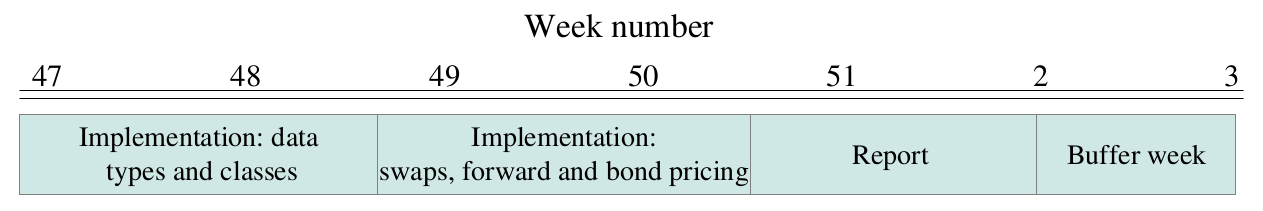
\includegraphics[bb = 0 0 1302 348, scale=0.275]{schedule.png}
\end{center}
\end{figure}

% REFERENCES
\bibliographystyle{abbrv}
%\addcontentsline{toc}{section}{References}
\bibliography{hql}

\end{document}
